\documentclass[11pt, letterpaper, oneside]{article}     % use "amsart" instead of "article" for AMSLaTeX format
\usepackage{geometry}                           % See geometry.pdf to learn the layout options. There are lots.
\geometry{letterpaper}                                  % ... or a4paper or a5paper or ...
%\geometry{landscape}                           % Activate for rotated page geometry
%\usepackage[parfill]{parskip}                  % Activate to begin paragraphs with an empty line rather than an indent
\usepackage{graphicx}				% Use pdf, png, jpg, or eps§ with pdflatex; use eps in DVI mode
                                                                % TeX will automatically convert eps --> pdf in pdflatex
\usepackage{amssymb, tikz, amsthm, amsmath}
\usepackage{hyperref}
\usepackage{caption, subcaption}
\usepackage{multicol}
\usepackage{enumitem}
\usetikzlibrary{decorations.pathreplacing}
\usepackage{geometry}
 \geometry{
 letterpaper,
 total={210mm,297mm},
 left=20mm,
 right=20mm,
 top=20mm,
 bottom=20mm,
 }
\pagestyle{empty}
\usepackage{colortbl}
%SetFonts

\theoremstyle{definition}
\newtheorem{theorem}{Theorem}
\numberwithin{theorem}{section}
%\newtheorem*{defi}{Definition}
%\newtheorem{defino}{Definition}
\newtheorem{defi}[theorem]{Definition}
\newtheorem{lemma}[theorem]{Lemma}
\newtheorem{cor}[theorem]{Corollary}
%\newtheorem*{cor}{Corollary}
%\newtheorem{cornum}{Corollary}
\newtheorem{prop}[theorem]{Proposition}
\newtheorem*{claim}{Claim}
\newtheorem*{ex}{Example}
\newtheorem*{quiz}{Quiz Question}

\theoremstyle{remark}
\newtheorem*{remark}{Remark}
\newtheorem*{note}{Note}
\newtheorem{notenum}{Note}
\newtheorem*{fact}{Fact}
\newtheorem*{sol}{Solution}
\newtheorem{exer}[theorem]{Exercise}
\newtheorem{exerset}[theorem]{Exercise Set}


%%%
%%% These are just a bunch of shorthand commands I like to define to make my life easier
%%% because I use them a lot.
%%%
\newcommand{\ZZ}{\mathbb{Z}}
\newcommand{\NN}{\mathbb{N}}
\newcommand{\RR}{\mathbb{R}}
\newcommand{\CC}{\mathbb{C}}
\newcommand{\PP}{\mathbb{P}}
\newcommand{\QQ}{\mathbb{Q}}
\newcommand{\FF}{\mathbb{F}}
\newcommand{\ds}{\displaystyle}
\newcommand{\abs}[1]{\lvert #1 \rvert}
\newcommand{\floor}[1]{\lfloor #1 \rfloor}
\newcommand{\ceil}[1]{\lceil #1 \rceil}
\newcommand{\dotp}{\boldsymbol{\cdot}}
\newcommand{\tth}{\textsuperscript{th}}
\newcommand{\ov}[1]{\overline{#1}}
\newcommand{\lcm}{\textrm{lcm}}

\title{MATH 342 Notes}
\author{Matthew Hinton}
\date{\today}

\begin{document}

\maketitle

\section{First Order Vector-Valued ODE}

\subsection{Repeated eigenvalues}

\begin{enumerate}[itemsep=10pt]
\item Example: Find a fundamental set for
  $\dot x = \begin{bmatrix} 1 & -1 \\ 4 & 5\end{bmatrix}x$.
  \begin{align}
    \lambda &= 3,\quad \xi = [1,-2]^T\\
    (d/dt-\lambda)^2 x &= 0 \text{ has solns } Ce^{\lambda t},\, Cte^{\lambda t}\\
  \end{align}
  Propose
  \begin{align}
    x = te^{\lambda t}\xi\,?
  \end{align}
  but then
  \begin{align}
    \dot x - Ax = e^{\lambda t}\xi \neq 0
  \end{align}
  so $x$ is not a solution.

  However, we can cancel off the nonhomogeneous part with an ansatz solution $e^{\lambda t}\eta$, $\eta \in \RR^2$, to the nonhomogenous equation $\dot x - Ax = e^{\lambda t}\xi$. (Compare with method of undetermined coefficients.)

  So
  \begin{align}
    x = te^{\lambda t}\xi - e^{\lambda t}\eta.
  \end{align}

  Then $\dot x - Ax = 0$ gives
  \begin{align}
    0 = e^{\lambda t}\xi + (\lambda e^{\lambda t}\eta - Ae^{\lambda t}\eta),
  \end{align}
  and therefore
  \begin{align}
    e^{\lambda t}(\xi + \lambda\eta - A\eta) = 0
    &\implies \xi + \lambda\eta - A\eta = 0\\
    &\implies \xi = (A - \lambda I)\eta.
  \end{align}
  Notice that $A - \lambda I$ is not invertible. But concretely we want to solve
  \begin{align}
    \begin{bmatrix}
      -2 & -1\\
      4 & 2
    \end{bmatrix}
    \begin{bmatrix}
      \eta_1 \\ \eta_2
    \end{bmatrix}
    =
    \begin{bmatrix}
      1 \\ -2
    \end{bmatrix}.
  \end{align}
  Is $\xi$ always in the column space of $A - \lambda I$?

\item Summary (choice of a fundamental set).

  \emph{In general} when $A$ has repeated eigenvalues, and $A$ is $2\times 2$,
  \begin{align}
    x^1 &= e^{\lambda t}\xi,\quad
    x^2 = te^{\lambda t}\xi + e^{\lambda t}\eta,
  \end{align}
  where $\eta$ is a solution to $(A-\lambda I)\eta = \xi$.

  $\eta$ is called a \emph{generalised eigenvector}.

  \emph{Highly important result}. If $\eta$ is \emph{any} vector independent of $\xi$, we will have $(A - \lambda I)\eta = c\xi$ for some $c \neq 0$. (Why?)

  \end{enumerate}

\subsection{Nonhomogeneous system}
\begin{enumerate}
  \item The system of interest is
  \begin{equation}\label{eq:nonhomogeneous-system}
    \dot x = P(t)x + g(t),\quad\quad P(t) \in M_{n\times n}(\RR),\quad x(t),g(t) \in M_{n\times 1}(\RR)
  \end{equation}
  Solution is given as a sum of a particular solution with a general solution of the corresponding homogeneous system (which we have already done). We will focus on finding particular solutions $x_p$ to (\ref{eq:nonhomogeneous-system}).

\item Methods:
  \begin{enumerate}
  \item Undetermined coefficients for special $g(t)$
  \item Laplace transforms
  \item Decoupled systems for diagonalizable $A$
  \item \textbf{Variation of parameters} (we will use this one)
  \end{enumerate}

  \underline{Example:}
  $\dot x = \begin{bmatrix} 1 & -1 \\ 4 & 5\end{bmatrix}x + \begin{bmatrix} e^t \\ 0 \end{bmatrix}$.

\item
  Proposed solutions (VOP):
  \begin{equation}
    x(t) = u_1(t)x^1(t) + u_2(t)x^2(t) \quad\quad\text{(undetermined coefficients)}
  \end{equation}
  where $u_1,u_2$ are scalar valued and $x^1$,$x^2$ solve the homogeneous equation. The goal is to find $u_1,u_2$.
  \begin{enumerate}
  \item Rewrite
    \begin{align}
      x(t) &=
      \begin{bmatrix}
        x^1(t) & x^2(t)
      \end{bmatrix}
      \begin{bmatrix}
        u_1(t) \\ u_2(t)
      \end{bmatrix}\\
      &= \Psi(t)u(t)\\
      &=
      \begin{bmatrix}
        e^t & e^{5t}\\
        -3e^t & e^{5t}
      \end{bmatrix}
      \begin{bmatrix}
        u_1(t) \\ u_2(t)
      \end{bmatrix}
    \end{align}

  \item Apply $x(t) = \Psi(t)u(t)$ to $\dot x(t) = Ax(t) + g(t)$ to get
    \begin{equation}\label{eq:cond_on_VOP_coeffs}
      \Psi'(t)u(t) + \Psi(t)u'(t) = A\Psi(t)u(t) + g(t)
    \end{equation}

  \item Remember $\Psi(t)$ is invertible, and also explicitly
    \begin{align}
      \Psi(t) &=
      \begin{bmatrix}
        x^1(t) & x^2(t)
      \end{bmatrix}\\
      \Psi'(t) &=
      \begin{bmatrix}
        Ax^1(t) & Ax^2(t)
      \end{bmatrix}\\
      &= A\Psi(t).
    \end{align}
    $\Psi$ solves a ``matrix version'' of the original homogeneous equation. We use this result to simplify (\ref{eq:cond_on_VOP_coeffs}):
    \begin{align}
      \Psi(t)u'(t) = g(t).
    \end{align}

  \item We have
    \begin{align}
      \begin{bmatrix}
        e^t & e^{5t}\\
        -3e^t & e^{5t}
      \end{bmatrix}
      \begin{bmatrix}
        u_1'(t) & u_2'(t)
      \end{bmatrix}
      =
      \begin{bmatrix}
        e^t & 0
      \end{bmatrix},
    \end{align}
    so
    \begin{align}
      \begin{cases}
        e^tu_1'(t) + e^{5t}u_2'(t) = e^t\\
        -3e^tu_1'(t) + e^{5t}u_2'(t) = 0
      \end{cases}
    \end{align}
    A solution is
    \begin{align}
      \begin{cases}
        u_1'(t) = 1/4\\
        u_2'(t) = \frac{3}{4}e^{-4t}
      \end{cases}
    \end{align}

  \item Recover $u(t)$ from $u'(t)$.
    \begin{align}
      u(t) = \int u'(t)dt =
      \int
      \begin{bmatrix}
        \frac{1}{4} \\ \frac{3}{4}e^{-4t}
      \end{bmatrix}
      dt
      =
      \begin{bmatrix}
        \frac{1}{4}t \\ -\frac{3}{16}e^{-4t}
      \end{bmatrix}
      + c
    \end{align}

  \item One particular solution is
    \begin{align}
      x(t) = \left(\int_0^t\frac{1}{4}ds\right)
      \begin{bmatrix}
        e^t \\ -3e^t
      \end{bmatrix}
      +
      \left(\int_0^t\frac{3}{4}e^{-4s}ds\right)
      \begin{bmatrix}
        e^{5t} \\ e^{5t}
      \end{bmatrix}.
    \end{align}

  \end{enumerate}

\item \emph{Solution method in general.}

  \underline{Problem} $$\dot x(t) = P(t)x(t) + g(t).$$

  \underline{Corresponding homogeneous system} $$\dot x(t) = P(t)x(t),$$ solved by $$\dot x_h = P(t)x_h.$$

  \underline{Solution to the nonhomogeneous system} $$x(t) = \Psi(t)u(t)$$ (solve for $u(t)$).

  \underline{Equation for $u(t)$} $$\Psi'(t)u(t) + \Psi(t)u'(t) = P(t)\Psi(t)u(t) + g(t).$$
  OBSERVE that $\Psi'(t) = P(t)\Psi(t)$ (even in the nonconstant $P(t)$ case), so that
  $$\Psi(t)u(t) = g(t).$$
  Furthermore, \emph{$\Psi$ is invertible.} This is because of the whole Wronskian nonzero $\implies$ nonzero everywhere / diffeq's do not collapse the dimension of subspaces spanned by solutions thing.
  Thus
  \begin{align}
    u(t) &= \int \Psi(t)^{-1}g(t)dt\\
    \implies x_p(t) &= \Psi(t)\left(c + \int_0^t \Psi(s)^{-1}g(s)ds\right)\\
    &= \Psi(t)c + \int_0^t\Psi(t)\Psi(s)^{-1}g(s)ds,
  \end{align}
  (which is even the general solution to the original equation, with degree of freedom $c$ to be determined by initial conditions).

  \textbf{Special case:} $P(t) = A$ (constant). Then
  \begin{align}
    x(t) = e^{tA}x(0) = \int_0^te^{(t-s)A}g(s)ds \quad\quad\text{(Duhamel's formula)}
  \end{align}

\end{enumerate}

\section{Power Series Solutions to ODE}

\subsection{Basic power series tools}
\begin{enumerate}
\item Example.
  \begin{equation}\label{eq:power-series-function-ex}
    f(x) = \sum_{n=1}^\infty a_nx^n = \sum_{n=1}^\infty\frac{2^n}{n}x^n.
  \end{equation}
  \begin{enumerate}
  \item Find the radius of convergence.

    The radius of convergence of a power series $f(x) = \sum_{n=1}^\infty a_n(x-x_0)^n$ is a number $R \geq 0$ such that
    \begin{enumerate}
    \item $\forall x$ satisfying $|x - x_0| < R$, $f(x)$ converges absolutely (as in, $\sum_{n=1}^\infty |a_n||x-x_0|^n$ converges).
      \item $\sum_{n=1}^\infty a_n(x-x_0)^n$ diverges whenever $|x - x_0| > R$.
    \end{enumerate}
    $R$ is called the \emph{radius of convergence}.

    (Here $R = 1/2$ by the Ratio Test.)\\

    \underline{Tools for finding the radius of convergence}

    \textbf{The Root Test:} If $\ds\lim_{n\to\infty}|a_n|^{1/n}$ converges, then $\ds R = \frac{1}{\lim_{n\to\infty}|a_n|^{1/n}}$.

    For instance, (\ref{eq:power-series-function-ex}) gives
    \begin{equation}
      R = \frac{1}{\lim_{n\to\infty}(2^n/n)^{1/n}} = \frac{1}{\lim_{n\to\infty}2/n^{1/n}}= 1/2\quad\quad\text{since $n^{1/n}\to 1$}
    \end{equation}

    \textbf{The Ratio Test:} If $\ds\lim_{n\to\infty}\frac{|a_{n+1}|}{|a_n|}$ converges, then $\ds R = \frac{1}{\lim_{n\to\infty}\frac{|a_{n+1}|}{|a_n|}}$.

    In our example,
    \begin{equation}
      R = \frac{1}{\lim_{n\to\infty}\frac{2^{n+1}/(n+1)}{2^n/n}} = \frac{1}{\lim_{n\to\infty}2n/n+1}= 1/2.
    \end{equation}

    \bigskip

  \item Find $f'(x)$ (for meaningful $x$)

    As usual, differentiate term by term. If $f(x)$ is given by a power series $\sum_{n=0}^\infty a_nx^n$, then
    \begin{equation}\label{eq:power-series-function-derivative}
      f'(x) = \sum_{n=0}^\infty na_nx^{n-1} = \sum_{n=1}^\infty na_nx^{n-1}
    \end{equation}
    By making a change of variable $k = n-1$, and noticing that the first term drops out of the above series (because $n=0$), we have
    \begin{equation}\label{eq:derivative-power-series}
      f'(x) = \sum_{k=0}^\infty (k+1)a_{k+1}x^k.
    \end{equation}
    This procedure for getting the power series into the desired powers of $x$ is called \emph{index shifting}. It is important to keep track of the initial value for $k$ and $n$ in the sum. This is analagous to changing the bounds of integration when performing a change of variable.

    A remarkable feature of the radius of convergence is that it is \emph{invariant under differentiation or integration of the power series}. Consider our example. Differentiating term by term or using (\ref{eq:derivative-power-series}), the derivative series is
    \begin{equation}
      f'(x) = \sum_{k=0}^\infty (k+1)\frac{2^{k+1}}{k+1}x^k
      = \sum_{n=0}^\infty 2^{n+1}x^n.
    \end{equation}
    By the ratio test, the radius of convergence of $f'(x)$ is
    \begin{equation}
      R = \frac{1}{\lim_{n\to\infty}\frac{2^{n+2}}{2^{n+1}}}
      = \frac{1}{2},
    \end{equation}
    which is the same as the radius of convergence for $f(x)$. The radius of convergence of the integral power series $\int dx f(x)$ is a fun exercise (it should also be $1/2$).

  \item \underline{Some notions.} Let
    \begin{equation}
      f(x) = \sum_{n=0}^\infty a_n(x-x_0)^n \quad\quad\text{with}\quad\quad R>0.
    \end{equation}
    \begin{enumerate}
    \item $f(x)$ is \emph{analytic} at $x = x_0$. (This is what it means to be analytic at $x_0$; there exists a convergent power series equal to the function on a neighborhood of $x_0$.)
    \item $a_n = f^{(n)}(x_0)/n!$, and $f(x) = a_0 + a_1(x - x_0) + a_2(x - x_0)^2 + \dots$, and in particular $f(x_0) = a_0$.
    \item Taylor series expansion: When $f$ is analytic at $x_0$, it has a particular power series representation for $f(x)$, given by
      \begin{equation}
        f(x) = \sum_{n=0}^\infty \frac{f^{(n)}(x_0)}{n!}(x-x_0)^n
      \end{equation}
      For example, the exponential function is its own derivative and $e^0 = 1$. This is enough to define the exponential everywhere by its Taylor series at $x_0 = 0$:
      \begin{equation}
        e^x = \sum_{n=0}^\infty \frac{(e^x)^{(n)}\big|_{x=0}}{n!}x^n = \sum_{n=0}^\infty \frac{e^0}{n!}x^n = \sum_{n=0}^\infty \frac{1}{n!}x^n,
      \end{equation}
      which should look familiar.

    \end{enumerate}

  \end{enumerate}

\item Analytic vs infinitely differentiable functions.

  \underline{Question:} Every function that is analytic at $x=0$ is infinitely differentiable at $x=0$. Is the converse true? NO!

  \underline{Example:}
  A classic example is the function $f:\RR \to \RR$ given by
  \begin{equation}
    f(x) =
    \begin{cases}
      e^{-1/x^2}, & x > 0\\
      0, & x \leq 0
    \end{cases}
  \end{equation}
  This function is infinitely differentiable at $x_0 = 0$ (why?) but is not analytic there. For if it were analytic, its Taylor series would be identically zero since $f^{(n)}(0) = 0$ for all $n$ (look at the value of $f$ for negative $x$ arbitrarily close to zero).

  \begin{center}
    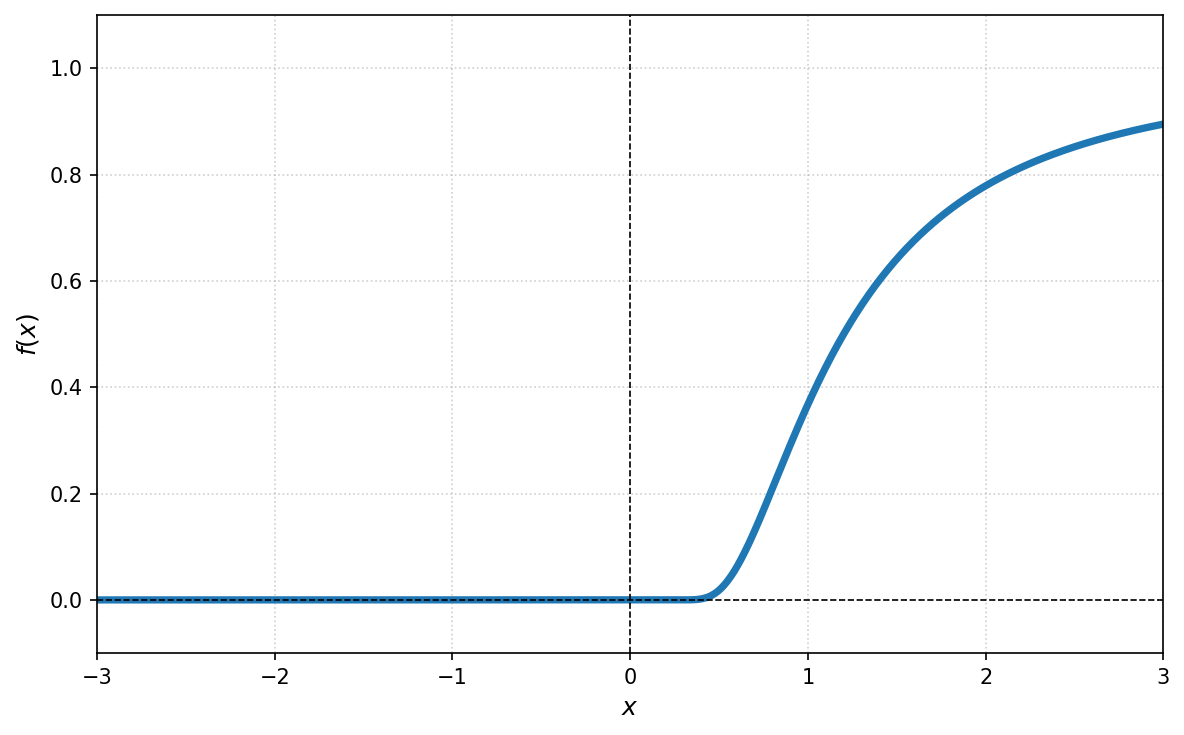
\includegraphics[width=0.8\textwidth]{nonanalytic_function}
  \end{center}

  \underline{Fact:} $\sum_{n=0}^\infty a_nx^n = 0 \implies a_n = 0$ for all $n$. This is just a restatement of what we said above. (If you define $f(x)$ by that power series then we identify the $a_n$ with the derivatives of $f$, which are all zero since $f$ is by assumption identically zero.)

\end{enumerate}

\subsection{Homogeneous DE with variable coefficients}

Consider the general type of ordinary differential equation
\begin{equation}\label{eq:homogeneous-de-with-variable-coeff}
  P(x)y'' + Q(x)y' + R(x)y = 0\quad\quad (y = y(x) \text{ is real valued})
\end{equation}
We will make the following assumption.

\underline{Assumption:} $P,Q,R$ are polynomials and there is no scalar $c$ such that $P(x),Q(x),R(x)$ are all divisible by $(x-c)$ (they are essentially ``coprime'' as elements of the ring of polynomials over the real or complex numbers).

\begin{enumerate}
\item Well known equations.
  \begin{enumerate}
  \item Airy's equation:
    \begin{equation}
      y'' - xy = 0,\quad\quad P(x) = 1, Q = 0, R(x) = -x.
    \end{equation}
  \item Bessel's equation:
    \begin{equation}
      x^2y'' + xy' + (x^2 - \nu^2)y = 0,\quad\quad P(x) = x^2, Q(x) = x, R(x) = x^2 - \nu^2
    \end{equation}
    where $\nu$ (the Greek letter ``nu'') is a parameter in the equation.

    If $\nu \neq 0$, then our assumption (about the coprime nature of $P,Q,R$) is satisfied, but not if $\nu = 0$. In the case $\nu = 0$, the equation simplifies a fair bit.

  \item Legendre's equation:
    \begin{equation}
      (1 - x^2)y'' - 2xy' + \alpha(\alpha + 1)y = 0,
    \end{equation}
    where $\alpha$ is a parameter.

  \end{enumerate}

\item Solution methods.

  Let us restate our DE in \textbf{standard form}.
  \begin{equation}
    y'' + \frac{Q}{P}(x)y' + \frac{R}{P}(x)y = 0
  \end{equation}
  or
  \begin{equation}
    y'' + p(x)y' + q(x)y = 0,
  \end{equation}
  where $p(x) = \frac{Q}{P}(x)$, and $q(x) = \frac{R}{P}(x)$.

  But wait! We need to verify that it is okay to divide by $P(x)$ (what if we are dividing by zero?). If $P(x_0) \neq 0$, then $P(x) \neq 0$ for all $x$ near $x_0$, and the standard form is valid near $x_0$. In this situation, $x_0$ is called an \textbf{ordinary point}.

\item \underline{Example:} Airy's equation.
  \begin{equation}\label{eq:airys-eq-example}
    y'' - xy = 0 \quad\quad (x\in\RR)
  \end{equation}
  We can do some quantitative analysis on Airy's equation and make some rough sketches of various solution curves to (\ref{eq:airys-eq-example}). This essentially boils down to using the equation to guess the sign and magnitude of $y''$ at different points on the sketch, and deducing the shape of the solution by forcing it to be consistent with this data. Unfortunately I can't draw in \LaTeX, so refer to the course notes for details.

  To proceed with the solution we use a power series ansatz
  \begin{equation}
    y(x) = \sum_{n=0}^\infty a_n(x-x_0)^n = \sum_{n=0}^\infty a_nx^n
  \end{equation}
  where $x_0 = 0$.

  Solving the (\ref{eq:airys-eq-example}) amounts to determining the coefficients $a_n$. To do this we need to plug $y(x)$ into (\ref{eq:airys-eq-example}). Let's calculate the derivatives (see the short section on power series):
  \begin{align}
    y'(x) &= \sum_{n=0}^\infty \frac{d}{dx}\left[a_nx^n\right]\\
    &= \sum_{n=1}^\infty na_nx^{n-1}\\
    y''(x) &= \sum_{n=1}^\infty \frac{d}{dx}\left[na_nx^{n-1}\right]\\
    &= \sum_{n=2}^\infty n(n-1)a_nx^{n-2}.
  \end{align}
  The lower limit of the sums is \emph{very important}. We drop terms when they are zero so that we don't end up with $x$ to negative powers in the derivative (e.g. $na_n = 0$ when $n=0$).

  Plugging into the differential equation, we have
  \begin{align}
    \sum_{n=2}^\infty n(n-1)a_nx^{n-2} - x\sum_{n=0}^\infty a_nx^n &= 0\\
    \implies\sum_{n=2}^\infty n(n-1)a_nx^{n-2} - \sum_{n=0}^\infty a_nx^{n+1} &= 0
  \end{align}
  Doing some index shifting with $k = n-2$ in the first sum and $k = n+1$ in the second sum, we get
  \begin{align}\label{eq:airys-power-series}
    \sum_{k=0}^\infty (k+2)(k+1)a_{k+2}x^k - \sum_{k=1}^\infty a_{k-1}x^k &= 0.
  \end{align}
  Writing out the first few terms, you can convince yourself that we have
  \begin{align}\label{eq:expansion-of-airys-equation}
    (2a_2 + 6a_3x + 12a_4x^2 + 20a_5x^3 + \dots) - (a_0x + a_1x^2 + a_2x^3 + a_3x^4 + \dots) &= 0.
  \end{align}
  Now we can simply collect terms with the same powers of $x$ and require that all of the coefficients are zero. We can do this because $1$, $x$, $x^2$, $x^3$ $\dots$ are linearly independent functions on an \emph{interval} (they are naturally called the Taylor basis for polynomials and power series). Since we know that the resulting power series is zero for $x$ in an interval (this technically comes from our hypothesis that the ansatz $y(x)$ is a solution), we can use this to determine $a_n$ for all $n$.

  We could use (\ref{eq:expansion-of-airys-equation}) to determine $a_0,a_1,a_2,\dots$, but we would never find them all. So let's do it formally. From (\ref{eq:airys-power-series}), we have
  \begin{equation}
    2a_2 + \sum_{k=1}^\infty \left[a_{k+2}(k+2)(k+1) - a_{k-1}\right]x^k = 0,
  \end{equation}
  which gives us the equations
  \begin{equation}
    \begin{cases}
      2a_2 = 0,\\
      a_{k+2}(k+2)(k+1) - a_{k-1} = 0\quad\forall k\geq 1
    \end{cases}
  \end{equation}
  The first equation gives $a_2 = 0$, and the second can be arranged to be
  \begin{align}
    a_{k+2} &=  - \frac{a_{k-1}}{(k+2)(k+1)}\quad\forall k\geq 1\\
    \implies a_{k+3} &=  - \frac{a_k}{(k+3)(k+2)}\quad\forall k\geq 1.
  \end{align}
  So any coefficient determines the coefficient three terms later in the series $f(x)$. Once we have $a_0$, we can generate $a_3$, and then $a_6$, and so on. Naturally, the coefficients form three decoupled sequencies or ``chains''
  \begin{align}
    &a_0,a_3,a_6,a_9,\dots,a_{3n},\dots\\
    &a_1,a_4,a_7,a_{10},\dots,a_{3n+1},\dots\\
    &a_2,a_5,a_8,a_{11},\dots,a_{3n+2},\dots = 0
  \end{align}
  The last of these is constant zero because $a_2 = 0$. The other two are controlled by two free parameters $a_0$ and $a_1$. By computing a few of these $a_n$s you will quickly realise a pattern, which you can write down as an explicit formula for coefficients in the first two chains:
  \begin{align}
    a_{3n} &= \frac{a_0}{\prod_{k=1}^n(3k-1)(3k)}\\
    a_{3n+1} &= \frac{a_1}{\prod_{k=1}^n3k(3k+1)}
  \end{align}
  (recall the notation $\prod_{k=1}^n q_k = q_1\cdot q_2\cdots q_n$).

  With this information we can simplify our ansatz and obtain the general solution.
  \begin{align}
    y(x) &= \sum_{n=0}^\infty a_nx^{n}\\
    &= \sum_{n=0}^\infty a_{3n}x^{3n} + \sum_{n=0}^\infty a_{3n+1}x^{3n+1}\\
    &= \sum_{n=0}^\infty \frac{a_0}{\prod_{k=1}^n(3k-1)(3k)}x^{3n} + \sum_{n=0}^\infty \frac{a_1}{\prod_{k=1}^n3k(3k+1)}x^{3n+1}\\
    &= a_0y_1(x) + a_1y_2(x),
  \end{align}
  where $y_1(x)$ and $y_2(x)$ are the two linearly independent solutions given by the power series in the previous line. This completes the derivation of the general solution to Airy's equation.

  \underline{Radius of convergence}
  Remember that power series functions are only defined within their radius of convergence. Let's check where our solution to the Airy's equation is actually defined!

  For $y_1(x)$,
  \begin{equation}
    b_n = \frac{a_0}{\prod_{k=1}^n(3k-1)(3k)}
  \end{equation}
  and so by the Ratio test
  \begin{align}
    R &= \frac{1}{\lim_{n\to\infty}\frac{|b_{n+1}|}{|b_n|}}\\
    &= \frac{1}{\lim_{n\to\infty}\frac{\prod_{k=1}^n(3k-1)(3k)}{\prod_{k=1}^{n+1}(3k-1)(3k)}}\\
    &= \frac{1}{\lim_{n\to\infty}\frac{1}{(3n-1)(3n)}}\\
    &= \infty.
  \end{align}
  This means our power series converges everywhere and we have a solution on the whole real line.

  As a final remark, we can imagine expanding the solution around some other point $x_0 \neq 0$. If we do this, we get faster convergence around the new $x_0$, which is important for numerical applications. In addition, we can imagine situations in which $R < \infty$, in which case it would be necessary to find power series solutions around a collection of points; these solutions can in some cases be ``patched together'' to get a solution on a larger domain than just $[-R,R]$.


\end{enumerate}

\end{document}
